\chapter{Travaux réalisés}


\section{Appréhension des données}


La base de données de \emph{Corine Land Cover} met à disposition deux types de données : des données raster et des données vector.
Dans cette section, je décris l'exploration que j'ai réalisée sur ces deux types de données.

\subsection{Données raster}

Les données raster sont constituées d'une matrice de zones carrées, des pixels, dont la taille détermine le détail qui peut être conservé dans le jeu de données.
La valeur d'un pixel peut être continue ou catégorielle représentant par exemple respectivement l'altitude ou l'utilisation des terres.
Ce type de donnée est notamment utilisé pour décrire l'intérieur des entités cartographiques et pour stocker des données qui varient continuellement d'un endroit à l'autre comme l'altitude, la température ou le pH du sol.


Les données raster de \emph{Corine Land Cover} sont constitués d'une unique bande représentant la catégorie de terrain de chaque pixel.
Un code RGB est associé à chacune des catégories de terrain.

% Une partie du raster complet, centrée sur Paris, peut être visualisée sur la figure 1.

\begin{figure}
% IMAGE RASTER
    \centering
    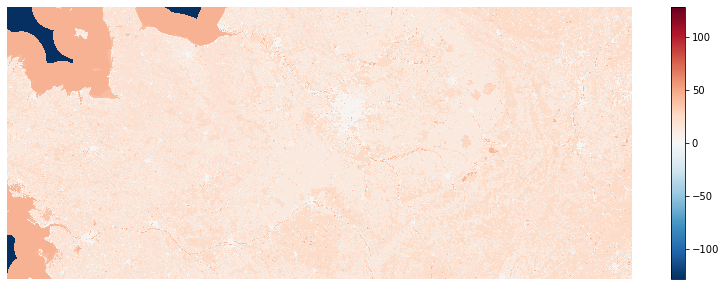
\includegraphics[scale=0.5]{figures/raster}
    \caption{Partie des données raster centrée sur le milieu de la France}
\end{figure}

\subsection{Données vector}


Les données vector sont constituées de coordonnées $x$ et $y$ pour définir la forme et l'emplacement des zones correspondant aux entités cartographiques.
Un vecteur peut être un point, une ligne ou un polygone représentant par exemple respectivement un point d'intérêt, une route ou un lac.
Ce type de donnée est notamment utilisé pour décrire le centre et les bords des entités et pour stocker des détails spatiaux.


Comme pour les données raster, les données vector de \emph{Corine Land Cover} sont constitués du type de terrain de chaque vecteur.


% Une partie des vecteurs, centrée sur Paris, peut être visualisée sur la figure 2.


\begin{figure}
% IMAGE VECTOR
    \centering
    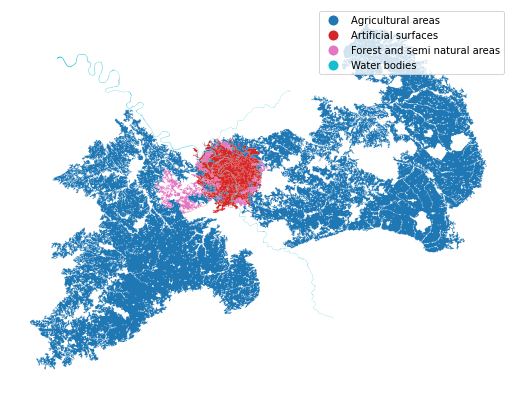
\includegraphics[scale=0.5]{figures/vector}
    \caption{Partie des données vectorielles centrée sur Paris}
\end{figure}

\subsubsection{Prélèvement automatique de zones géographiques}

L'extraction manuelle de zones de vecteurs à l'aide de logiciels tels que \emph{QGIS} est fastidieuse et peu précise.
C'est pourquoi il est nécessaire d'avoir un moyen d'automatiser le processus.

Le module \emph{Python} \emph{GeoPy}, intégré au sein du module \emph{Geopandas}, permet de convertir un nom en coordonnées géographiques.
À partir de ce point, nous pouvons créer une surface avec un certain rayon et extraire la partie du jeu de données complet qui lui correspond à l'aide de la fonctionnalité dédiée dans \emph{Geopandas}.
Cette dernière extrait toutes les surfaces en contact avec la zone d'extraction.


\begin{figure}
% IMAGE AIRE PRELEVEMENT AUTOMATIQUE ZONE
    \centering
    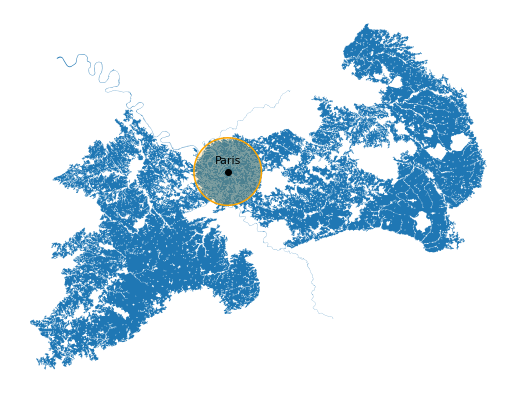
\includegraphics[scale=0.5]{figures/zone-paris}
    \caption{Construction d'une surface pour le prélèvement automatique d'une zone}
\end{figure}



Un exemple de prélèvement automatique peut être visualisé sur la figure 3.
Dans cet exemple, nous construisons une surface centrée sur Paris pour prélever une zone similaire de celle présentée sur la figure 2.

\subsubsection{Vérification des ordres de grandeur}

Afin de définir si des informations relatives aux longueurs des vecteurs sont exploitables, il est nécessaire de vérifier si leur ordre de grandeur semble correcte.

Pour ce faire, nous vérifions les longueurs calculées des vecteurs sur une zone dont on connaît les dimensions.
Par exemple, le lac d'Annecy.
Grâce à l'outil de prélèvement automatique décrit précédemment, nous extrayons sa zone correspondante et nous calculons son périmètre : nous obtenons un écart de $2,6\%$.
Cet écart est satisfaisant, c'est pourquoi nous considérons que les longueurs calculées sur les vecteurs sont correctes et peuvent être utilisées pour l'apprentissage.

%\begin{figure}
%% IMAGE LAC ANNECY
%\centering
%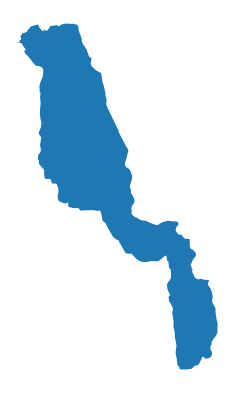
\includegraphics[scale=0.5]{figures/annecy}
%\caption{Instance du jeu de données de \emph{Corine Land Cover} correspondant au lac d'Annecy prélevée automatiquement à partir de son nom}
%\end{figure}

\subsection{Association raster - vector}

Il aurait été intéressant d'associer les données raster aux données vector.
En effet, les rasters auraient pu servir de complément d'information, telles des images, notamment grâce aux codes RGB présentes dans ces dernières.
Cependant, une valeur RGB n'est pas associée à chaque pixel, mais à une catégorie de terrain.
Cela rend donc leur intérêt moindre.
Les données raster ne semblent donc finalement pas intéressante à exploiter.

% Le découpage du raster en fonction d'un vecteur spécifique peut être visualisé en figure 3.


\section{Construction des jeux de données pour la classification de graphes}


Dans l'objectif de faire de l'apprentissage pour la classification de graphes, il convient de construire et de préparer des jeux de données adéquats en amont.
Dans cette section, je décris la construction des différents jeux de données qui seront utilisés pour l'apprentissage.

\subsection{Capitales et campagnes}

Dans ce premier jeu de données, nous voulons extraire de la base de données \emph{Corine Land Cover} des capitales et des campagnes, dans le but de les classifier.

\subsubsection{Sélection des capitales et des campagnes}

J'ai alors recensé des capitales d'Europe de tailles similaires : Berlin, Madrid, Helsinki, Paris, Rome, Varsovie, Bucarest, Londres, Stockholm.
Pour les campagnes, j'ai collecté manuellement 36 points dans des grandes zones rurales.
Les campagnes étant de manière générale plus vastes et homogènes que les villes, ces points ont été collectés de manière aléatoire sur le territoire recouvert par la base de données \emph{Corine Land Cover}.

\subsubsection{Choix de la taille d'extraction}

Le choix de la taille de la zone d'extraction est crucial pour construire un jeu de données en adéquation avec ce que l'on veut collecter.
Dans le cas des capitales, l'objectif est d'extraire des zones qui représentent au mieux les espaces urbains.
On ne veut donc pas inclure de terrains définissant des zones rurales.
Il faut donc choisir une taille de zone assez grande pour avoir un nombre d'instances suffisant pour l'apprentissage, mais pas trop grande pour ne pas récupérer la périphérie des plus petites villes.

C'est pourquoi j'ai relevé la répartition des catégories de terrain pour plusieurs tailles d'extraction.
L'objectif est de choisir celle dont la répartition correspond le mieux au type de région qu'on souhaite extraire : urbain pour les capitales et rural pour les campagnes.
Comme les campagnes sélectionnées sont plus vastes que les villes, la contrainte sera exclusivement imposée par les capitales.
La figure 5 présente la répartition des catégories de terrain pour des tailles d'extraction de 10 à 100 km² pour les capitales.


\begin{figure}
% IMAGE REPARTITION TERRAINS EN FONCTION DE LA TAILLE D'EXTRACTION
    \centering
    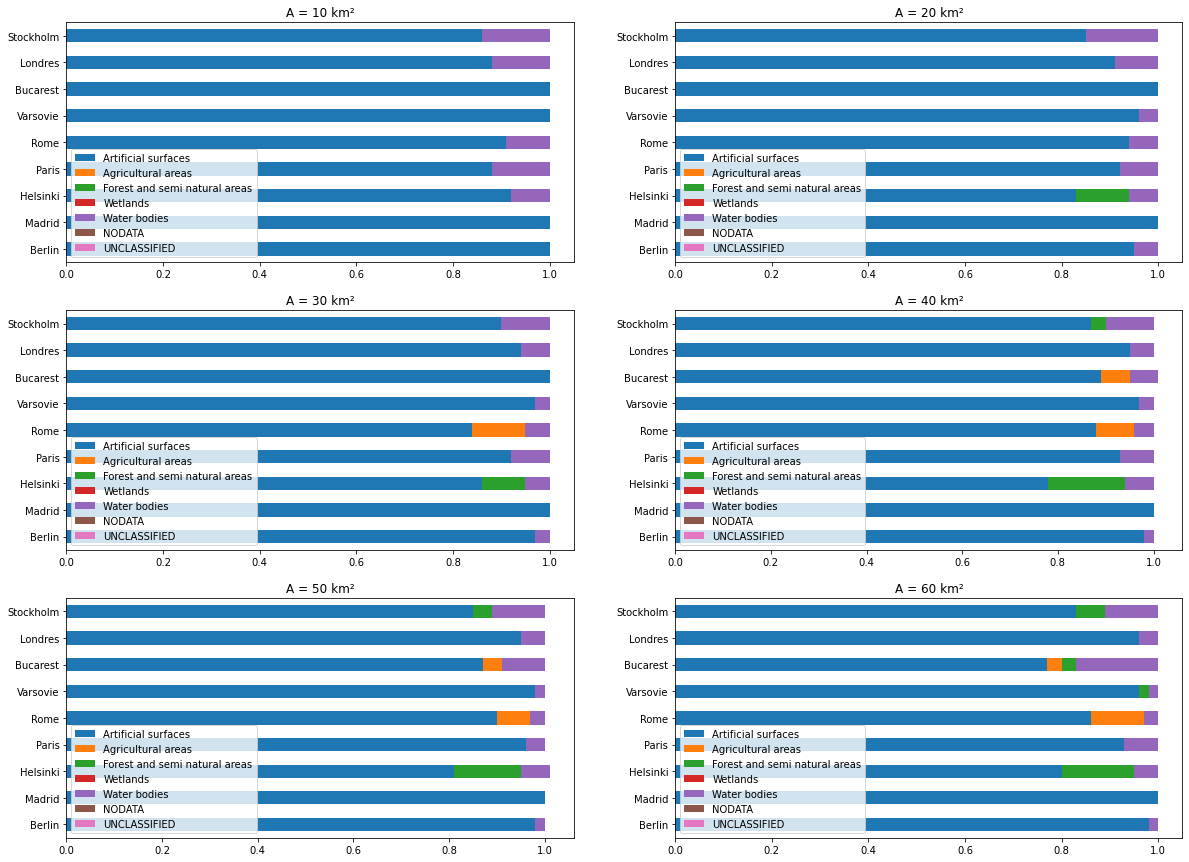
\includegraphics[width=\textwidth]{figures/taille-extraction}
    \caption{Répartition des types de terrains en fonction de la taille d'extraction $A$ pour la création du jeu de données des capitales}
\end{figure}



La taille d'extraction retenue est alors de 20 km².
Cette dernière permet de maximiser le taux de parcelles urbaines dans le jeu de données tout en conservant un nombre important d'instances.
Il sera peut-être nécessaire, en fonction des résultats de l'apprentissage, d'augmenter ce rayon ou d'utiliser plus de villes pour avoir plus d'instances.

\subsection{Communes de France}

Dans ce second jeu de données, nous souhaitons extraire de la base de données \emph{Corine Land Cover} environs 5000 communes de tailles similaires, dans le but de les classifier de manière non supervisée.
Pour ce faire, nous utilisons la base de données des communes de France.

\subsubsection{Sélection des communes}

L'objectif est de sélectionner environs 5000 communes avec des tailles similaires.
Remarquons que $75\%$ des exemples présents dans le jeu de données des communes de France ont une surface inférieure à $2000$ hectares.
La figure 7 montre la répartition des surfaces des communes, parmi celles ayant une surface inférieure à $3000$ hectares.
Nous sélectionnons des communes dont la taille n'est pas trop petite pour maximiser les chances d'y trouver des zones urbaines dans la base de données \emph{Corine Land Cover}.
Nous prenons donc les communes avec une surface comprise entre 1900 et 3000 hectares.
Il s'agit donc de petites communes rurales.

\begin{figure}
% IMAGE REPARTITION DE LA TAILLE DES COMMUNES
    \centering
    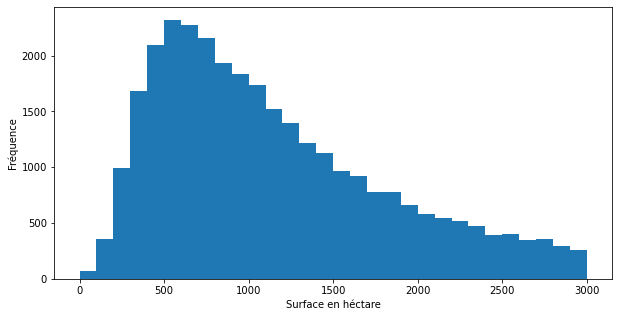
\includegraphics[scale=0.5]{figures/surf-communes}
    \caption{Répartition de la surface des communes parmi celles ayant une surface inférieure à 3000 hectares}
\end{figure}

\subsubsection{Extraction des zones géographiques}

Afin d'extraire les zones géographiques correspondant aux communes, nous pouvons directement appliquer un masque dans la base de données \emph{Corine Land Cover} à partir des communes de la base de données des communes.
La figure 8 présente le découpage de la commune Eyne par ce procédé.

\begin{figure}
% IMAGE DECOUPE BRUTE OLETTA
    \centering
    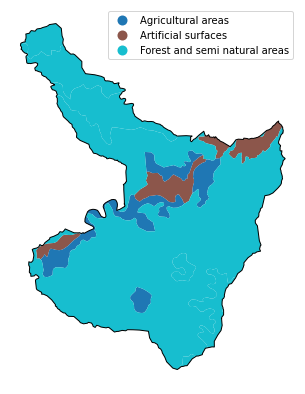
\includegraphics[scale=0.5]{figures/eyne-decoupe-brute}
    \caption{Extraction de la commune d'Eyne dans les données de \emph{Corine Land Cover} à partir de celles des communes de France}
\end{figure}

Cependant, nous pouvons observer qu'un tel découpage peut séparer des aires de \emph{Corine Land Cover} en plusieurs parties distinctes. On souhaite alors les décomposer en instances séparées.

\begin{figure}
% IMAGE REDEFINITION DES AIRES COUPEES OLETTA
    \centering
    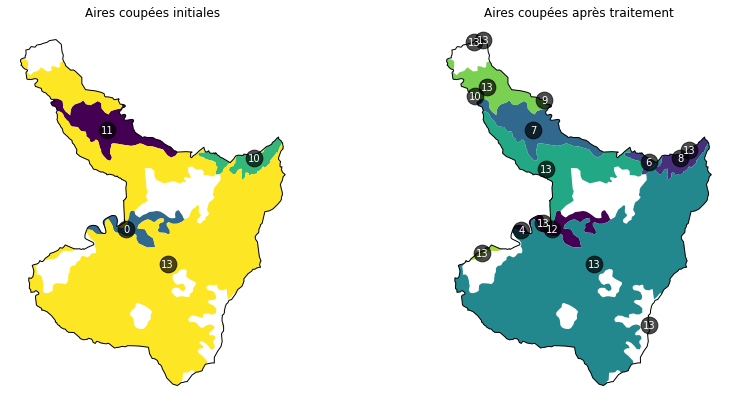
\includegraphics[scale=0.5]{figures/eyne-redef-aires}
    \caption{Redéfinition des aires coupées après extraction pour la commune d'Eyne}
\end{figure}



Enfin, le découpage fait apparaître des aires résiduelles aux extrémités de la carte.
Ces dernières ne sont pas représentatives de la zone que l'on souhaite extraire et peuvent donc constituer un biais pour l'apprentissage.
Nous souhaitons donc les supprimer.
Nous calculons alors la proportion de la taille conservée des surfaces et la proportion de la taille totale des surfaces après découpage.
Nous pourrons ainsi fixer par la suite un seuil pour ne conserver que les surfaces représentatives.
Ces proportions sont présentées pour la commune d'Eyne sur la figure 9 et la figure 10 montre un exemple de suppression de ses aires résiduelles en fixant les seuils respectifs à $40\%$ et $1\%$ .


\begin{figure}
% IMAGE PROPORTION OLETTA
    \centering
    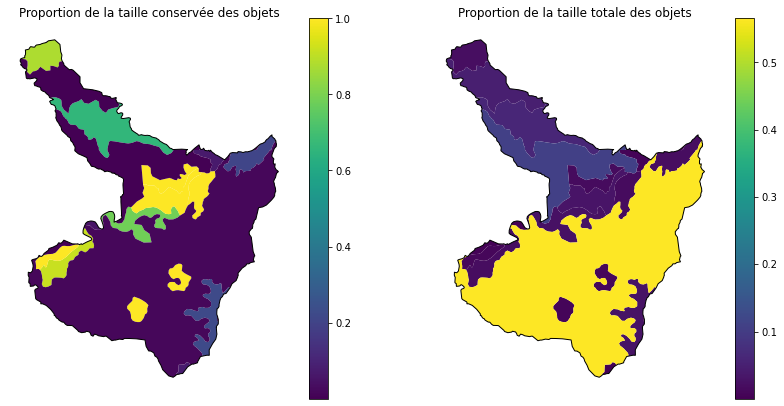
\includegraphics[scale=0.5]{figures/eyne-residus-prop}
    \caption{Proportions de la taille conservée et de la taille totale des objets après extraction pour la commune d'Eyne}
\end{figure}


\begin{figure}
% IMAGE SUPPRESSION AIRES RESIDUELLES OLETTA
    \centering
    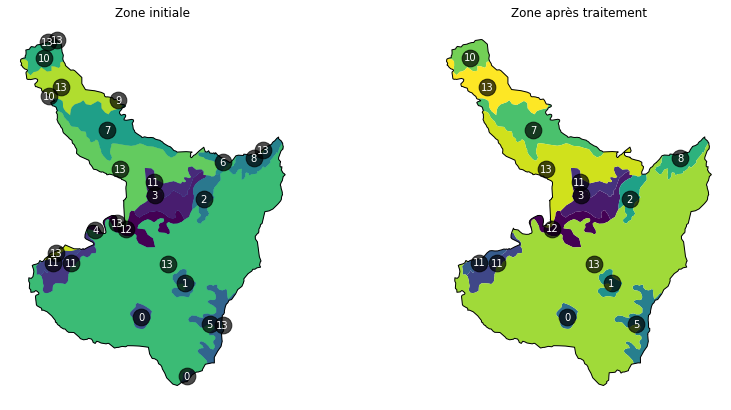
\includegraphics[scale=0.5]{figures/eyne-sup-residus}
    \caption{Exemple de suppression des aires résiduelles après extraction pour la commune d'Eyne}
\end{figure}


\section{Construction des graphes}


% Dans cette section, je décris la création des graphes à partir des jeux de données construits précédemment.

%\subsection{Définition des graphes}


% Cette partie décrit de quelle manière un graphe permet de représenter une zone géographique.


Un graphe représente une zone géographique de la manière suivante.
Un noeud du graphe correspond à une surface dans le jeu de données de \emph{Corine Land Cover}.
Il contient à la fois des informations géométriques telles que l'aire et le périmètre de la surface, et des informations sémantiques telles que le type de terrain associé à la surface.
Deux noeuds sont alors voisins si leurs surfaces correspondantes dans le jeu de données sont voisines.
Il convient donc dans un premier temps de définir la notion de voisinage. %Des informations supplémentaires pourront être portées par les arrêtes en fonction de caractéristiques émanantes de cette définition.

L'idée est de vérifier si des surfaces voisines dans les données de \emph{Corine Land Cover} se touchent forcément, ou si elles peuvent être légèrement éloignées.
Pour ce faire, on calcule la distance entre paire de surfaces et on vérifie si, en dessous d'un certain seuil, il existe ou non une autre surface entre les deux.
Si tel est le cas pour l'intégralité des exemples tester, on peut considérer que les surfaces voisines se touchent toutes.
Sinon, il faudra considérer une éventuelle distance entre paire de surfaces voisines.
Sur 12 zones extraites du jeu de données initiale, avec en moyenne 600 surfaces par zone et en fixant un seuil à $100$ mètres, il n'y a aucune paire de surfaces dans ce deuxième cas.

Nous définissons donc des surfaces voisines dans les données de \emph{Corine Land Cover} comme des surfaces qui se touchent, et une arête du graphe met en évidence cette relation de voisinage.
Le calcul du voisinage pour créer le graphe se fait alors naïvement en récupérant pour chaque surface des données, toutes les surfaces qui la touchent.
Des informations supplémentaires peuvent ensuite être portées par les arrêtes du graphe comme la taille de la frontière entre deux surfaces voisines.
Puisque ces frontières peuvent être discontinues, le nombre de frontières, la taille de la plus grande frontière et la somme des tailles des frontières sont également des informations portées par les arrêtes.
La figure 11 montre un exemple de graphe construit avec cette méthode sur la commune d'Eyne.


\begin{figure}
% IMAGE SUPPERPOSITION GRAPHE - MAP
    \centering
    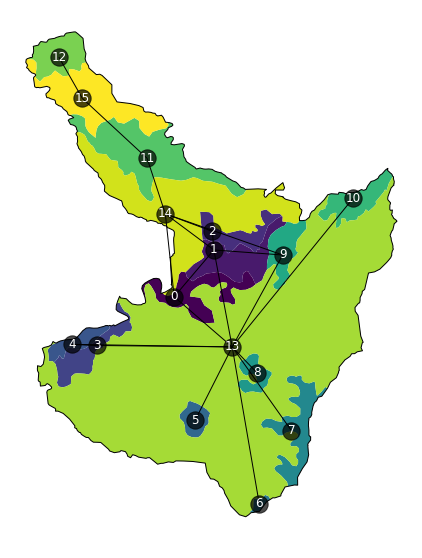
\includegraphics[scale=0.5]{figures/eyne-map-graph}
    \caption{Graphe associé à la commune d'Eyne}
\end{figure}







